

\chapter{Theory}
\label{chap:theandme}
This chapter is divided into two parts. The first part explains general deep learning and natural language processing basics, with a focus of this work in mind. The second part of this chapter offers a more detailed explanation of methods relevant to this work.

\section{General Background}


\subsection{Linguistics and Natural Language Processing}

%začni větou Historie počítačoví lingvistiky se datuje v..... hlavně se zabývali překladem a vyhledáváním v textu. V současné době
Linguistics is a science which describes language and its focus can be divided into following sub-fields:
\begin{itemize}
\item phonetics
\item phonology
\item  morphology
\item syntax
\item semantics
\item pragmatics
\end{itemize}

%ZDROJ jirka hana
This work is focused on task belonging into morphology, syntax and semantics. 

\textbf{Morphology} studies internal structures of words. Basic building block of a word is a morpheme and such morphemes can represent semantics (meaning) or grammatical role of the world. %TODO příklad
One word can occur many forms created via inflection. %todo like apple - apples, 
Such a set of all possible forms is called lexeme. Morphology is eldest lingusitical field %TODO zdroj, 
early automated models for morphological language processing focused on generating forms from lemmas %TODO zdroj, Two level morphology
Czech morphology developement is dated from 1989 %TODO zdroj Hajič.
and in description uses 15-places morphological tags. %TODO obrázek 
Morphology is used for many tasks, which can be divided into generation and analysis. Results of a morphological analysis is a set of possible lemmas and tags for given word form. This set can be further narrowed by lemmatization (selection of one "right" lemma), morphological tagging (selection of one right tag in given context), partitional disambiguation (removes all tags and lemmas, which can be reliably removed). Morphology can be also used for tasks like automatic spell check, text searching, key words tagging %TODO system asimut, mosaica %TODO nebo?
Lemmatization task consist of finding a \textit{lemma} - lemma is one chosen form of a word, selected to represent whole lexeme set. It is chosen by a convention -- (i.e. noun it is nominative of singular, for verb its infinitive). Czech is synthetic mostly fusional language (?).

\textbf{Syntactic analysis} goes beyond the boders of words and studies sentence structure. %TODO obrazek stromů
Different word classes play different roles in a sentences. For example noun can be object %TODO 
or subject, verb is typically %TODO přísudek
, but can serve as a %TODO podmět.
Sentence structure can be describe using various combinations of trees, generatig rules and sets of tags. %TODO obrazky a příklady
Part of speech %TODO
Syntactic analysis is used for text generation, machine translation, grammatical checks. %TODO další

Historical development of computer linguistics was significantly affected by machine translation. First attempts started in 1933 by patents for machien translation %TODO zdroje!!!
which leaded to big boom in the 50s and 60s and than to a slowdown after ALPAC report in 1966. %TODO zdroje
In current times, not only machine translation systems but many other linguistic taks solving by machine learning methods, which often leads to better results with less need of expert knowledge in comparison to complicated sets of rules used before. %TODO zdroj?
\par
%korpusy - k čemu to je, jak to navazuje na to předchozí
Useful tools for the study of languages are corpuses. A corpus is a large collection of texts, which aims to be in some way representative sample of a language (this is of course not fully possible, but can help). In addition to 

\par

The history of learning algorithms inspired by a human brain started in the 1940s under the name \textit{cybernetics} \citep{Goodfellow-et-al-2016} \citep{McCulloch}.
Perceptron \citep{Rosenblatt1958}, found in 1957, is the simplest neural network with just one layer serving for binary classification (see Fig. \ref{pic:perceptron}).

\begin{figure}[ht]
\centering
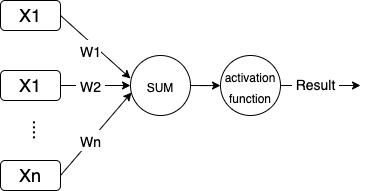
\includegraphics[width=0.8\columnwidth]{../img/perceptron}
\caption{A one-layer perceptron architecture. The result is formed by the application of activation function on a weighted sum of inputs. Weights are updated during training till it returns satisfactory results. }
\label{pic:perceptron}
\end{figure}
There also exists a multi-class version for the general classification. The problem of this perceptron was the inability to classify data that are not linearly separable \citep{Minsky2017} (see Fig. \ref{pic:xor}), which led to a lack of interest in deep networks for some period.
\begin{figure}[ht]
\centering
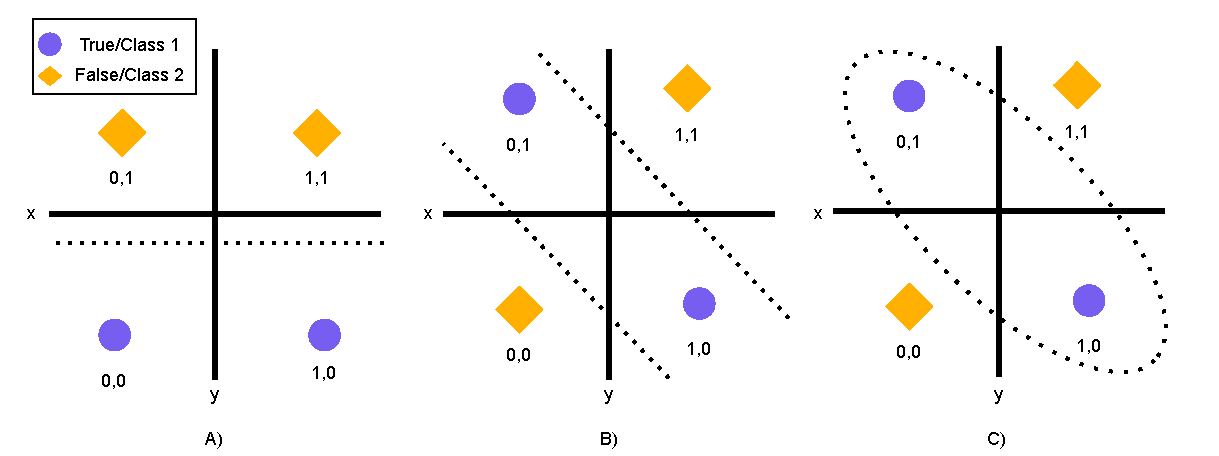
\includegraphics[width=1\columnwidth]{../img/xor}
\caption{This picture illustrates XOR problem. Perception can find the correct solution only if the data are linearly separable. It means, that they can be divided by a hyperplane. An example of such two-dimensional data can be seen in picture A). The dotted line shows a possible border for separation. Picture B) shows XOR problem. XOR is a logical operation on two boolean variables, which returns true if one variable is True (1) and the other one is False (0), and returns False otherwise. Such data cannot be separated by one hyperplane. Linearly non-separable data can be for example separated by a circle (pic. C)}
\label{pic:xor}
\end{figure}
\par
\textit{Deep} neural networks era started in 2007 with bigger datasets and greater computational resources. These two new features opened the possibility of neural network learning without expertly handcrafted parameters tuning with good results.
Some now frequently used ideas are quite old, like the perceptron or a back-propagation algorithm, and are combined with better choice of activation functions, some ideas appeared in the last two decades -- like convolutional neural networks or encoders.
\par
%TODO NLP ... cíle, tasky
The basic type of DNN is a multilayer perceptron (see picture %todo picture).
It is combined with neurons, every neuron has an activation function, which is applied to its input. Input to every, but the first layer is a weighted combination of (possibly selection of) previous layer neurons. 
Different types of NN differs by number and shape of layers, activation functions and connections between neurons. (see Fig. \ref{pic:multilayer}).
\begin{figure}[ht]
\centering
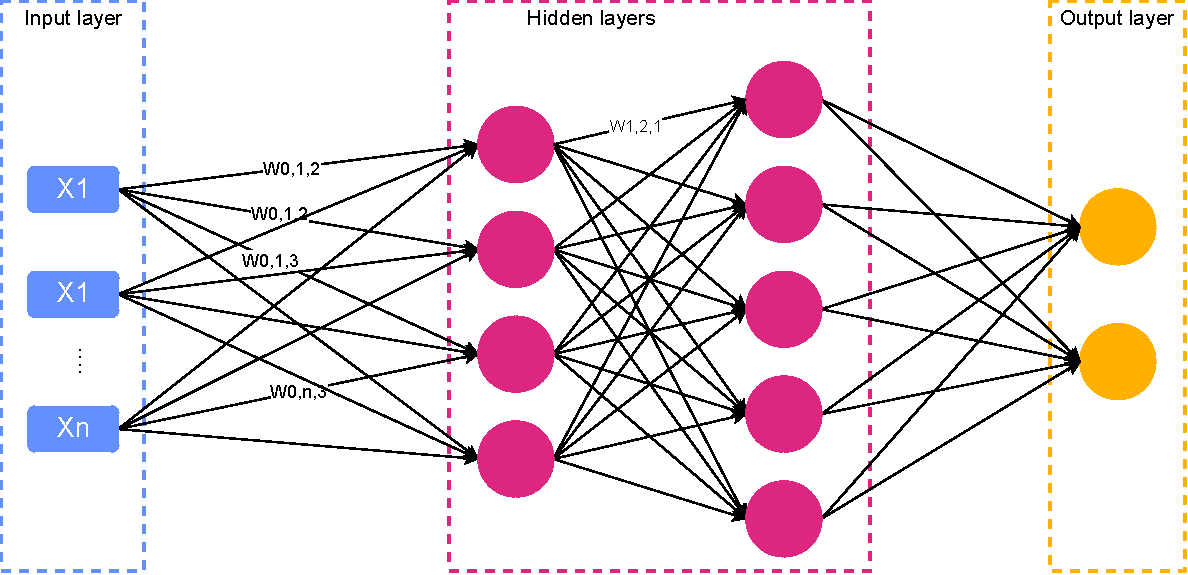
\includegraphics[width=1\columnwidth]{../img/multilayer}
\caption{Multilayer perceptron (or feed-forward neural network) is formed input and outpu layer and variable number of hidden layers with different sizes. In every layer, chosen application function is applied to a weighted sum of inputs from previous layer.}
\label{pic:multilayer}
\end{figure}

Some of the key ideas for (not only) NLP and specifically for BERT, are presented in the following subsections.

%v dalsi casti vysvetlim nektere nove vylepseni z poslednich let, ktere vedly k vyraznemu improvementu (nejen) v oblasti NLP.
\subsection{Label smoothing}
Supervised machine learning problems can be distinguished by the desired outcome as classification or regression. Classification means that we want to sort data into one of predefined classes, meanwhile regression is some numerical result. In the case of multi-class classification, true results (labels) can be in one of following forms -  text or number mark or one-hot vector. If there are more than two classes presented, one-hot vector has length equal to number of classes and consist of zeros on every indices but target class index, where is one. %TODO see picture
Label smoothing is an idea applicable to every classification problem, therefore is not limited to a NLP only. %todo zdroj
In any classification task, training data contains labels of the correct classes. In binary classification or one-hot encoded labels, correct class is denoted by 1 and incorrect class(es) by 0. Instead of this, label smoothing applies following formula: 
$$y_{new} = (1 - \epsilon) * y + \alpha / K$$, where $K$ is number of classes. Label smoothing is used as a cure for overfitting and overconfidence in the case of use of a softmax 
 as output activation function. Loss function for softmax classification is: 
 $$ loss = -\sum_{i=1}^{n} \sum_{y=1}^{K} p(y \mid x_i) log \, q_{\theta} ( y_i \mid x_i ) $$
 and after substitution of label smoothing\footnote{Taken from: https://leimao.github.io/blog/Label-Smoothing/}:
$$
loss_{ls} = -\sum_{i=1}^{n} \sum_{y=1}^{K} [(1-\epsilon) p(y \mid x_i)+\epsilon u(y\mid x_i)]log \, q_\theta(y \mid x_i) $$,
which gaves after multiplication\footnote{Taken from: https://leimao.github.io/blog/Label-Smoothing/}:

 \begin{equation} \label{eq:lsloss}
 loss_{ls}= \sum_{i=1}^{n} {(1- \epsilon)[- \sum_{y=1}^{K} p(y\mid x_i) log \, q\theta(y \mid x_i)]+\epsilon [- \sum_{y=1}^{K} u(y \mid x_i)log \, q\theta (y\mid x_i)]}
 \end{equation}
 
From equation \ref{eq:lsloss} can be seen, than if the network is very confidential about some prediction, second part of loss function is very large, so label smoothing works as a regularization of overconfidence.


\subsection{Attention mechanism}
\label{sub:attention}
%používá se i v grafice
Attention mechanism is widely used in NLP as a tool for extracting relevant informations from word sequences. For example when generating translation of some sentence, each word in target language corresponds to just few words in source sentence, not to a whole sentence. Attention gives weights to the words, which represents this connections. When the task is a question answering %todo zdroj, 
attention can help a model to focus on relevant part in the text, where the answer is allocated. For example see picture %TODO obrazek.
Modification to this concept, called self-attention, deals with relationships inside one part of text (like a sentence). This variant of attention do not connect one part of text (like question) to other different part of text (like answer), but only models relationships inside one sentence. %TODO obrazek z videa a poradne vysvetlit
Attention has three inputs -- key, value and query, all vectors. The output is weighted sum of values and the weights are computed with respect to key-query pair. 


%%%%%%%%%%%%%%%%%%%%%%%%%%%%%%%%%GRU, LSTM, Transformers
\subsection{Recurrent Neural Networks}
Human language has a sequential nature. Word and sentences ordering is an important part of text and lack of it can make text absolutely nonsense. This places hard demands on neural networks, because such data structure differs from most of other NN applications, where input samples are independent and ordering does not matter. Second problem connected to such sequential processing is vanishing/exploding gradient. %TODO vysvetlit
Text sequences can be very long and information from more distant words, which is relevant for given word, can vanish or explode very easy. %todo obrázek s příkladem věty

The construction of such networks, which are able to capture natural language structure requires solving two problems:
\begin{itemize}
\item input should be understood by network as a sequence,
\item there must be a possibility to use information from other parts of sentence (or text).
\end{itemize}
 First problem was solved by simple Recurrent Neural Networks (RNN) %todo picture with explanation
, while the latter problem needed more complicated approach. There are basically three attempts to solve this \textit{short memory} of RNN cells -- Gated Recurrent Unit (GRU), Long Short Term Memory (LSTM) and Transformers architecture with attention mechanism.
\par
Both LSTM and GRU uses an idea of gating. Gates works as weights for previous informations and new input. They help to decide which information should be remembered and which should be forgotten. %todo obrazek gates 
%vysvetlit detailne
\subsubsection*{LSTM} LSTM cell uses input, output and forget gate. Every gate is composed by sigmoid function with actual input and previous hidden state as inputs. %see picture 
%see picture with gates and equations!
%todo nomenclature
%http://colah.github.io/posts/2015-08-Understanding-LSTMs/
\subsubsection*{GRU}
GRU also uses gates: reset gate and update gate. %todo obrzek s popisem.
Reset gate is responsible for how much of previous state will take in the new state. Update gate is then weight for a combination for previous and current states, which together form new output.

\subsection{Transformers}
A Tranformers architecture was proposed in a paper Attention Is All You Need %todo cite
and essentially depends on textbf{attention} mechanism (see subsection \ref{sub:attention}). In the example of sentence processing, attention in nutshell is able to tell us which other words are important while determining something about currently processed word.
Tranforems uses encoder-decoder architecture, which was simultaniously proposed in 2014 by two papers. The basic idea behind this architecture is following: encoder and decoder are connected by some middle layer of fixed size which aims to be good representation of an input. Encoder reads its input and tries to learn such weights, that encoder's final representation of the input contains all important information. Decoder has this representation as its input and tries to produce best results. It was first use for machine translation, so the output of the encoder in this case is a sentence in the target language with same semantics as original input. %todo obrazek s popisem ze to je sekvence
Transformers are novelty in the manner that there are no LSTM cells computing hidden states.%pravda?
Picture %todo z clanku 
describes design of one layer. Both encoder and decoder are built by many blocks of respective type. Self-attention mechanism which is supposed to select most important words to be focused on is used on many places -- for input of every encoder layer, input of every decoder layer (although masked) and also between encoder and decoder. On the decoder side, self-attention layer is masked so the decoder can "see" just previous words (there are $-inf$ values in the positions on the right side). For representation of word position in the sentence (as it is not RNN cell and it can process all words simultaneously) Transformers uses position embeddings, which are trained to represent the ordering in the sentence.
%fixed length vector
%recurrent and shortuct links,normalization



\subsection{Embeddings}
Good performance of NLP models relies on text representation. What is hypothetically deserved is teaching computers to understand semantics of language. Once computer has a good representation of what given text \textit{means}, it should be easy to answer questions, translate into another language etc. Because NN are able to work only with numerical representation of inputs, second requirement upon such language representation is to be numerical. Straightforward way is to represent input words in one-hot encoding. It means that single word is represented by vector where is only 1 at the position of respective word and all other positions are zeros.%todo obrazek
 Such vector is long as a number of distinct words in a dictionary, so it could be quite wide. Most important problem is that in this representation, every two words has same distance to each other. This is not true in linguistics. Words can have similar meanings, be opposite to each other etc.
\par
Better solution than one-hot encoding are embeddings. Embedding is a fixed-size vector, which represent input word. These embedding are not hand crafted by humans, they are learned by NN. They can be learned for every specific task from scratch or it is possible to use good pretrained embeddings. Before contextualized embeddings appeared, such pretrained embeddings were created mainly by Word2Vec, specifically by its two variants: CBOW and SkipGram model. %todo obrazek
CBOW model's objective is to predict a word from its context and SkipGram does exaty the oppposite - predicting context of a given word. These predicting objectives serves just as a tool for forcing a network to learn useful word representation. There is an embedding layer at the beggining of the network with size $number\_of\_words \times embedding\_size$. Word2Vec-like embeddings uses just few context words and they does not use explicitly information about statistics in whole dataset. GloVe %todo zdroj
embeddings on the other hand, uses information about frequencies of pairs of words in a whole dataset and are designed to project word vectors into meaningful vector space. 
\\
Embeddings of previously described types though uses context of the word -- it is in fact how they are meant to work. Similar words are supposed to appear frequently in similar context. Problem of such embedding is that a word has always same embedding independently of a context. This is definitely a problem in the case of homonyms, but contextualized embeddings showed to be generally better than traditional embeddings. %todo zdroje
That is why contextualized embeddings where invented in recent years %todo zdroj.
In addition to BERT, there is also GTP-2 and ELMo. Their comparison can be found in a subsection \ref{sub:specialBert}. 
\par
As embeddings are trained after the input is encoded into one-hot vectors, it is impossible to use pretrained embedding for encoding of previously unseen words. This is solved by embeddings of characters or subwords.


%%%%%%%%%%%%%%%%%%%%%%%%%%%%%%%%%%%%%%%%%%%Relevant methods
\section{BERT explanation}
This work mainly relies on Bidirectional Encoder Representations from Transformers (BERT)%todo zdroj
, so this section describes and explains main mechanisms of this model. 
The core of BERT algorithm is based on these three features -- two unsupervised task for pretraining, input and its embeddings, transformers encoder %todo ref
architecture.

\subsection{Input embeddings}
%todo obrazek
BERT uses concatenation of three types of embeddings as an input representation -- token embeddings, position embeddings and segment embeddings. %todo figura z berta

\subsubsection*{Token embeddings}
Input of BERT model can be one or two word sequences (not necessarily two sentences, but e.g. also paragraphs). All words are split into tokens and converted into embeddings with a use of pretrained embeddings model. One word can be tokenized into more tokens as WordPieces %todo zdroj
embeddings are used. WordPiece pretrained embedding algorithm was originaly created for task of Google voice search for Asian languages and is designed to minimize occurence of unknown word tokens. This model was not pretrained as a part of BERT paper experiments, but represents quite interesting solution, so I will briefly explain the idea. In the first iteration of training, the model creates embeddings only for basic characters. In every other iteration, some existing model words are concatenated together in the way that cause the highest likelihood of input text. As a result of this method, some words will be embedded as one word and some will be split into more tokens as can be seen on figure. %todo obrazek
\par
There are three other tokens which are added after this step -- CLS, END, SEP. 
CLS token is added at the beginning of the input and is used as first sequence embedding for classification tasks (as sentence analysis). SEP token separates both sequences and END token is appended at the end. Whole input transformation can be seen on figure %todo dodat obrazek.

\subsubsection*{Position embeddings}
All input tokens are processed simultaneously, so there is no information about order of tokens. However, nature of the language is sequential, bunch of words without an order has no language meaning so there are position embeddings for this. They have same shape as token embeddings (and also as segment embeddings), so concatenation with two other types is easy.

\subsubsection*{Segment embeddings}

%todo tyhle jsou asi trenovane :o
These emebddings just indicates whether the token belongs to first or second part of input. It has same dimension as position and token embeddings.

\subsection{Pretraining tasks}
%todo narozdil od jinych modelu co jsou trenovane jednosmerne blabla...
BERT is pretrained on two unsupervised tasks -- Next Sentence Prediction (NSP) and Masked LM (MLM). These two tasks were chosen specifically because BERT's authors belief they can force language model to learn general and useful knowledge about language. 

\subsubsection*{Next Sentence Prediction}
Input of the BERT model for this task are two sentences A ans B. In 50\% of cases, sentence B is sentence which really follows sentence A in the text. Otherwise it is random sentence from the text. A goal of the task is decision whether sentence B is following or random, i.e. binary classification. Motivation for this task is a need to represent relationships between sentences, not only between words. Experiments showed its usefulness for text tasks as question answering. Last hidden representation of CLS token, therefore its representation in last hiddne layer, is used for prediction. %todo obrazek

\subsubsection*{Masked Language Modeling}
Masked Language Modeling or Cloze taks (%todo zdroj)
consist of prediction of some missing words in text. In the case of BERT, its implementing in the following way: 15\% of tokens in each sequence are chosen. For each of this chosen tokens there is 80\% chance to be replaced by MASK token, 10\% chance to by replaced by random token or it will remain unchanged with 10\% probability. This ensures, that the model will try to predict tokens not only in the case of MASK token presence. For backpropagation, only predictions of MASK token are taken into account. Prediction is done by softmax which input is last hidden representation of respective token. This prediction is done with informations about both sides context, which is main difference from other preceding language models. How exactly is this allowed will be described in the architecture section.

\subsection{Transformers encoder architecture}
BERT adapts encoder part of architecture from orginal Transformers paper %todo zdroj. a odkaz na sekci v teorii
.
Actually, BERT uses this encoder architecture for each layer, 
%todo odkaz a vysvetlit
 o there is L (e.g. 12 in the case of BERT base model) encoder layers finished with one fully connected layer for specific task. In pretraining, there is only one layer responsible for MLM and NSP, as each task uses different part of last hidden layer informations. %todo obrazek architektury
 
 \subsection{Why is BERT so special?}
 \label{sub:specialBert}
 %napsat ze je special a proc -- vysledky, asi v teorii a odkaz dát sem
For deep learning architectures, it is quite common that reason why they work (especially why they work so well in comparison with other posibilities) is not visible at first sight. Authors offers following explanation. In contrast to other SOTA league language models, BERT uses both bidirectional context of words. In the figure %todo obrazek z berta
is a comaprison of two other such models - ELMo and GTP %todo zdroje
. GTP is also based on Transformers architecture, but unlike BERT, it uses decoder part of Transformer. 
GTP uses just left context of the word, as a sentence is proceeded sequentially. ELMo uses LSTM %todo odkaz
with both left-to-right and right-to-left training and concatenates results at the end. BERT is proceeding both sides context simultaneously and due to an architecture, in \textit{every layer} every transformer block has potentially information from every other block (and thus from every other word). That is the reason, why BERT is called \textbf{deeply} bidirectional or also non-directional (because there is no right-to-left or left-to-right direction of processing).
\par
Explanation of why and how BERT works are, however, not so simple. There are many papers on how BERT works, what BERT really learns and know, how BERT architecture can be simplyfied and so on. There actually appeared new term "bertology" for this area of research.
 

